%%%%%%%%%%%%%%%%%%%%%%%%%%%%%%%%%%%%%%%%%%%%%%%%%%%%%%%%%%%%%%%%%%%%%%%%%%%%%%%%

\talksection{SPMD Execution Model}

\begin{frame}{SPMD Execution Model}

\begin{itemize}
    %\item Data-parallel
    %\begin{itemize}
    %    \item Work needs to be divided into chunks
    %\end{itemize}
    
    \item Single program
    \begin{itemize}
        \item Scalar form, but implicit SIMD execution
    \end{itemize}
    
    \item Multiple instances running in parallel
    \begin{itemize}
        \item Each instance working on a different data chunk
    \end{itemize}
    
    \item On GPU
    \begin{itemize}
        \item Divide work between lanes of SIMD units (fine division)
        \item SIMD execution in lockstep
    \end{itemize}
    
    \item On CPU
    \begin{itemize}
        \item Divide work between cores (coarse division)
        \item Sequential execution within a core (naive approach)
    \end{itemize}
\end{itemize}

%\begin{itemize}
%    \item Simplistic example:
%    \begin{itemize}
%        \item Massive Online Course
%        \item Compute the overall grade (GPA) of millions of students
%        \item GPA is the weighted average of several grades
%    \end{itemize}
%\end{itemize}

\end{frame}

%% Kernel function has no return value, takes in buffers (arrays)
%% Vectorization does not change the signature for kernels
%% Can also vectorize "normal" functions, but this results in signature changes

%%%%%%%%%%%%%%%%%%%%%%%%%%%%%%%%%%%%%%%%%%%%%%%%%%%%%%%%%%%%%%%%%%%%%%%%%%%%%%%%

\begin{frame}{Division of Work}

\begin{itemize}
    \item Work-item
    \begin{itemize}
        \item Unit of work
        \item One instance of a program
        \item Executed in parallel by Execution Units (threads)
    \end{itemize}
    \item Work Dimensions
    \begin{itemize}
        \item 1D (array shape)
        \item 2D (grid shape)
        \item ...
    \end{itemize}
\end{itemize}

\vspace{1ex}
\hspace{1em}
\includegraphics[scale=0.75]{images/work-items.pdf}

\end{frame}

%%%%%%%%%%%%%%%%%%%%%%%%%%%%%%%%%%%%%%%%%%%%%%%%%%%%%%%%%%%%%%%%%%%%%%%%%%%%%%%%

\begin{frame}[fragile]{Single Program}

\begin{itemize}
    \item Kernel function
    \begin{itemize}
        \item Entry point for the computation
    \end{itemize}
    \item Executed once per work-item
    \begin{itemize}
        \item As if there was a loop around it (but no dependency between iterations)
        \item Access to the iteration counter using \texttt{\varying{get\_global\_id(0)}}
    \end{itemize}
\end{itemize}

\vspace{1ex}
\begin{minipage}[t]{0.45\linewidth}
\begin{codebox}[commandchars=\\\[\]]
kernel void add_uniform(global int *dst,
                        global int *src,
                        int alpha) {
  int \varying[tid] = \varying[get_global_id(0)];
  dst\idx[\varying[tid]] = src\idx[\varying[tid]] + (alpha - 1);
}
\end{codebox}

\end{minipage}\hspace{1em}\begin{minipage}[t]{0.49\linewidth}
\begin{codebox}[commandchars=\\\[\]]
int *dst = ...;
int *src = ...;
int alpha = ...;
for (int \varying[tid] = 0; \varying[tid] < num_items; \varying[tid]++) {
  dst\idx[\varying[tid]] = src\idx[\varying[tid]] + (alpha - 1);
}
\end{codebox}

\end{minipage}

%\begin{codebox}
%kernel void calc_gpa(global *float result, global *int grades, global *float weights,
%                     int num_grades, int num_students) {
%    int student_id = get_global_id(0);
%    float gpa = 0.0;
%    for (int i = 0; i < num_grades; i++) {
%        int grade = grades[(i * num_students) + student_id];
%        float weight = weights[i];
%        gpa += (grade * weight);
%    }
%    result[student_id] = gpa;
%}
%\end{codebox}

\end{frame}

%%%%%%%%%%%%%%%%%%%%%%%%%%%%%%%%%%%%%%%%%%%%%%%%%%%%%%%%%%%%%%%%%%%%%%%%%%%%%%%%

\talksection{Vectorization}
\begin{frame}{Why Vectorize?}

\begin{itemize}
    \item Many executions units each executing one instance of a single program 
    \begin{itemize}
        \item Works well on GPU (many hardware threads)
        \item Not so much on CPU (very few cores)
        \item CPU has to execute many work-items sequentially
    \end{itemize}
    \item Speed up this sequential computation using SIMD units
    \begin{itemize}
        \item Vertical Vectorization
        \item Horizontal Vectorization
    \end{itemize}
\end{itemize}

\end{frame}

%%%%%%%%%%%%%%%%%%%%%%%%%%%%%%%%%%%%%%%%%%%%%%%%%%%%%%%%%%%%%%%%%%%%%%%%%%%%%%%%

\begin{frame}{Vertical Vectorization}

\begin{itemize}
    \item Patterns within a single work-item
    \begin{itemize}
        \item e.g. loops within a kernel
        %\item In our example, the weighted average computation
    \end{itemize}
    \item Using the LLVM Loop Vectorizer or SLP Vectorizer
    \item However, not all kernels contain vectorizable patterns
\end{itemize}

\vspace{2ex}
\hspace{1em}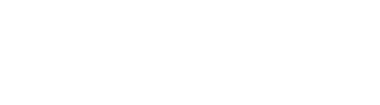
\includegraphics[scale=0.75]{images/vertical-vectorization.pdf}

\end{frame}

%%%%%%%%%%%%%%%%%%%%%%%%%%%%%%%%%%%%%%%%%%%%%%%%%%%%%%%%%%%%%%%%%%%%%%%%%%%%%%%%

\begin{frame}{Horizontal Vectorization}

\begin{itemize}
    \item Across work-items
    \begin{itemize}
        \item Compute multiple work-items at the same time
        \item Take advantage of the execution model (single program, multiple data)
    \end{itemize}
    \item Does not depend on special code patterns like loops
    \item SPMD Vectorizer
\end{itemize}

\vspace{2ex}
\hspace{1em}
\includegraphics[scale=0.8]{images/horizontal-vectorization.pdf}

\end{frame}

%%%%%%%%%%%%%%%%%%%%%%%%%%%%%%%%%%%%%%%%%%%%%%%%%%%%%%%%%%%%%%%%%%%%%%%%%%%%%%%%

\begin{frame}{SPMD Vectorizer}

\begin{minipage}[t]{0.45\linewidth}

\begin{itemize}
    \item Vectorizes a SPMD program's entry point function
    \item Given a function $F$ and vectorization factor $N$, produces a function $VF_N$
    \begin{itemize}
        \item Calling $VF_N$ is like calling $F$, but $N$ times (on consecutive work-items)
        \item $F$ and $VF_N$ have the same signature
    \end{itemize}
    
    \item The original function can be preserved (cloned) or not (in-place vectorization)
    \begin{itemize}
        \item Working on cloned function allows vectorization to fail gracefully
    \end{itemize}
    
    %\item Vectorization may be allowed to fail
    %\begin{itemize}
    %    \item On failure, the original function can be used 
    %\end{itemize}
\end{itemize}

\end{minipage}
\hspace{1em}
\begin{minipage}[t]{0.48\linewidth}

\vspace{0.1ex}
\center{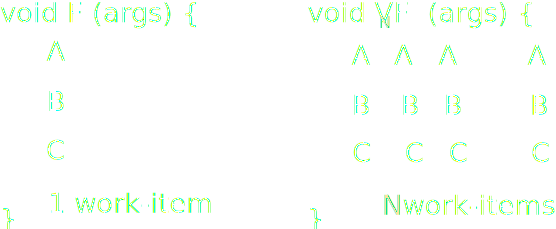
\includegraphics[width=\textwidth]{images/F-vs-VFn.pdf}}

\end{minipage}

\end{frame}

%%%%%%%%%%%%%%%%%%%%%%%%%%%%%%%%%%%%%%%%%%%%%%%%%%%%%%%%%%%%%%%%%%%%%%%%%%%%%%%%

%\begin{frame}{Vectorizer Comparison}
%
%\begin{itemize}
%    \item Loop Vectorizer
%    \begin{itemize}
%        \item Can be used for both vertical and horizontal vectorization
%        \item Has to enforce dependencies between loop iterations
%        \item Execution order is not specified, this is not needed
%        \item Nested control-flow?
%    \end{itemize}
%
%    \item SLP Vectorizer
%    \begin{itemize}
%        \item Finds groups of similar scalar instructions (same opcode)
%        \item Vertical vectorization
%        \item Not all kernels contain this kind of code
%    \end{itemize}
%
%    \item SPMD Vectorizer
%    \begin{itemize}
%        \item Only supports horizontal vectorization
%        \item Nested control-flow
%        \item Not limited to a certain 'style' of code
%    \end{itemize}
%\end{itemize}
%
%\end{frame}

%%%%%%%%%%%%%%%%%%%%%%%%%%%%%%%%%%%%%%%%%%%%%%%%%%%%%%%%%%%%%%%%%%%%%%%%%%%%%%%%

\begin{frame}{Glossary}

\begin{itemize}
    \item Work
    \begin{itemize}
        \item Work-item: unit of computation to execute in parallel.
        \item Instance: Code and state associated with one work-item.
        \item SIMD Lane: Execution of one instance of a vectorized kernel.
        \item SIMD Group: Contains all lanes that can be executed in parallel (at the same time).
        \item SIMD Width: Number of parallel lanes. Vectorization factor ($N$).
    \end{itemize}
        
    \item Data
    \begin{itemize}
        %\item Packet: Contains several values, one per SIMD lane. Maps to one value or instruction in the original kernel. Usually a vector instruction.
        %\item Packet: Maps a value in the original function to $N$ values, one per SIMD lane.
        \item Packet: $N$ values that map to $1$ value in the original function. One per SIMD lane.
        \item \uniform{Uniform}: Packet where values are identical for all lanes.
        \item \varying{Varying}: Packet where values are not identical for all lanes.
    \end{itemize}

    \item Control Flow
    \begin{itemize}
        \item \uniform{Uniform}: Branch taken by all lanes.
        %\item \varying{Divergent}: Conditional branch taken by only some lanes.
        \item \varying{Divergent}: Some lanes take one side of a branch, remaining lanes the other side.
    \end{itemize}
\end{itemize}

\end{frame}
